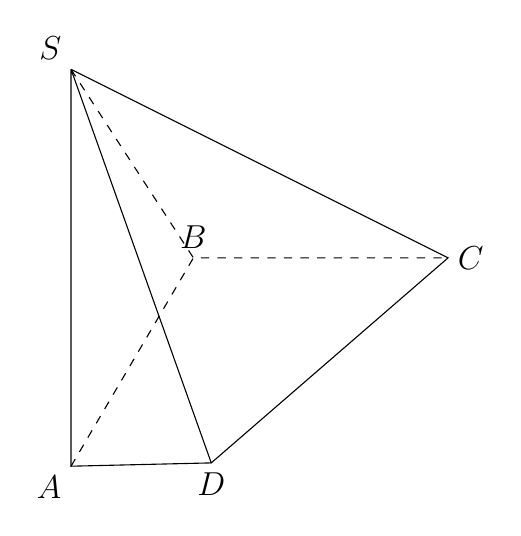
\begin{tikzpicture}[scale=.84, every node/.style={font=\large}]
  \coordinate (S) at (0,6.0);
  \coordinate (A) at (0,0);
  \coordinate (B) at (1.85,3.15);
  \coordinate (C) at (5.7,3.15);
  \coordinate (D) at (2.12,.05);
  \draw (S)--(A)--(D) (S)--(C)--(D)--(S);
  \draw[dashed] (A)--(B)--(C) (S)--(B);
  \node[above left] at (S) {$S$};
  \node[below left] at (A) {$A$};
  \node[above] at (B) {$B$};
  \node[right] at (C) {$C$};
  \node[below] at (D) {$D$};
\end{tikzpicture}
